% File tacl2021v1.tex
% Dec. 15, 2021

% The English content of this file was modified from various *ACL instructions
% by Lillian Lee and Kristina Toutanova
%
% LaTeXery is mostly all adapted from acl2018.sty.

\documentclass[11pt,a4paper]{article}
\usepackage{times,latexsym}
\usepackage{url}
\usepackage[T1]{fontenc}

% Chinese support
\usepackage{xeCJK}

% Graphics support
\usepackage{graphicx}

% TikZ for figures (optional, not needed for PNG figures)
% \usepackage{tikz}
% \usetikzlibrary{shapes,arrows,positioning,calc}


%% Package options:
%% Short version: "hyperref" and "submission" are the defaults.
%% More verbose version:
%% Most compact command to produce a submission version with hyperref enabled
%%    \usepackage[]{tacl2021v1}
%% Most compact command to produce a "camera-ready" version
%%    \usepackage[acceptedWithA]{tacl2021v1}
%% Most compact command to produce a double-spaced copy-editor's version
%%    \usepackage[acceptedWithA,copyedit]{tacl2021v1}
%
%% If you need to disable hyperref in any of the above settings (see Section
%% "LaTeX files") in the TACL instructions), add ",nohyperref" in the square
%% brackets. (The comma is a delimiter in case there are multiple options specified.)

\usepackage{tacl2021v1}
% \setlength\titlebox{10cm} % <- for Option 2 below

%%%% Material in this block is specific to generating TACL instructions
\usepackage{xspace,mfirstuc,tabulary}
\newcommand{\dateOfLastUpdate}{Dec. 15, 2021}
\newcommand{\styleFileVersion}{tacl2021v1}

\newcommand{\ex}[1]{{\sf #1}}

\newif\iftaclinstructions
\taclinstructionsfalse % AUTHORS: do NOT set this to true
\iftaclinstructions
\renewcommand{\confidential}{}
\renewcommand{\anonsubtext}{(No author info supplied here, for consistency with
TACL-submission anonymization requirements)}
\newcommand{\instr}
\fi

%
\iftaclpubformat % this "if" is set by the choice of options
\newcommand{\taclpaper}{final version\xspace}
\newcommand{\taclpapers}{final versions\xspace}
\newcommand{\Taclpaper}{Final version\xspace}
\newcommand{\Taclpapers}{Final versions\xspace}
\newcommand{\TaclPapers}{Final Versions\xspace}
\else
\newcommand{\taclpaper}{submission\xspace}
\newcommand{\taclpapers}{{\taclpaper}s\xspace}
\newcommand{\Taclpaper}{Submission\xspace}
\newcommand{\Taclpapers}{{\Taclpaper}s\xspace}
\newcommand{\TaclPapers}{Submissions\xspace}
\fi

%%%% End TACL-instructions-specific macro block
%%%%

\title{A Survey on Machine Translationese: \\From Corpus-Based Studies to Large Language Models}

% Author information does not appear in the pdf unless the "acceptedWithA" option is given

% The author block may be formatted in one of two ways:

% Option 1. Author’s address is underneath each name, centered.

\author{
  Template Author1\Thanks{The {\em actual} contributors to this instruction
    document and corresponding template file are given in Section
    \ref{sec:contributors}.} 
  \\
  Template Affiliation1/Address Line 1
  \\
  Template Affiliation1/Address Line 2
  \\
  Template Affiliation1/Address Line 2
  \\
  \texttt{template.email1example.com}
  \And
  Template Author2 
  \\
  Template Affiliation2/Address Line 1
  \\
  Template Affiliation2/Address Line 2
  \\
  Template Affiliation2/Address Line 2
  \\
  \texttt{template.email2@example.com}
}

% % Option 2.  Author’s address is linked with superscript
% % characters to its name, author names are grouped, centered.

% \author{
%   Template Author1\Thanks{The {\em actual} contributors to this instruction
%     document and corresponding template file are given in Section
%     \ref{sec:contributors}.}$^\diamond$ 
%   \and
%   Template Author2$^\dagger$
%   \\
%   \ \\
%   $^\diamond$Template Affiliation1/Address Line 1
%   \\
%   Template Affiliation1/Address Line 2
%   \\
%   Template Affiliation1/Address Line 2
%   \\
%   \texttt{template.email1example.com}
%   \\
%   \ \\
%   \\
%   $^\dagger$Template Affiliation2/Address Line 1
%   \\
%   Template Affiliation2/Address Line 2
%   \\
%   Template Affiliation2/Address Line 2
%   \\
%   \texttt{template.email2@example.com}
% }

\date{}

\begin{document}
\maketitle
\begin{abstract}
  The field of machine translation (MT) has undergone rapid evolution, with techniques advancing from statistical (SMT) and neural (NMT) paradigms to the recent dominance of Large Language Models (LLMs). A persistent byproduct of this technological progression is ``translationese''---systematic linguistic artifacts that distinguish machine-translated text from human-written text. The characteristics of translationese have co-evolved with MT systems, shifting from overt grammatical errors in early models to more subtle biases such as simplification, normalization, and excessive literalism in modern NMT and LLM outputs. This paper surveys this research landscape, reviewing the progression of methods for the detection, characterization, and mitigation of translationese. 
  %Finally, we highlight ongoing challenges and future directions for managing this phenomenon in an era of ubiquitous MT.
\end{abstract}

\section{Introduction}

The field of machine translation (MT) has undergone a dramatic evolution, advancing from rule-based systems to the sophisticated Large Language Models (LLMs) of today. This progression, marked by milestones such as phrase-based Statistical MT (SMT) \cite{koehn2003statistical}, the attention mechanism in Neural MT (NMT) \cite{bahdanau2015neural}, and the Transformer architecture \cite{vaswani2017attention}, has significantly enhanced translation quality and accessibility. However, a persistent byproduct of this technological advancement is ``translationese''---systematic linguistic artifacts that distinguish translated text from text originally authored in the target language \cite{gellerstam1986translationese}. Understanding the nature and evolution of translationese is not merely an academic exercise; it is critical for improving MT systems, ensuring fairness, and mitigating long-term risks such as the degradation of training data.

Translationese is not a monolithic phenomenon; its characteristics have co-evolved with MT paradigms. Early corpus-based studies, building on foundational concepts like translation universals \cite{baker1993corpus}, identified general features such as simplification (reduced lexical diversity) and normalization (adherence to typical target language patterns) in human-translated texts \cite{laviosa1998corpus}. The SMT era brought a focus on source-language interference, with researchers demonstrating that ``source language markers''---subtle linguistic patterns influenced by the source text---could be used to identify the original language of a translation with high accuracy \cite{koppel2011translationese,van2008source}. This discovery highlighted that even statistically optimized systems carry traces of their source material.

The advent of NMT, while reducing overt grammatical errors, introduced more subtle biases. These include a continued loss of lexical richness \cite{vanmassenhove2019getting}, a tendency towards more conservative and less creative language use, and the emergence of ``post-editese,'' a hybrid artifact found in human-edited NMT outputs that retains some machine-like qualities \cite{toral2019post}. Most recently, LLMs have been shown to produce their own distinct form of translationese. While capable of highly fluent output, they often exhibit excessive literalism, a phenomenon where the model adheres too closely to the source text's structure, and a strong tendency to ``over-normalize'' text, smoothing out stylistic variations \cite{li2025how,wang2024benchmarking}. These subtle artifacts can be difficult for human evaluators to detect but can have significant downstream effects.

In response to this evolving challenge, a substantial body of research has developed methods to monitor, document, and mitigate the effects of translationese. The task of detecting translationese has progressed from manual analysis and feature-based classifiers, which relied on hand-crafted linguistic features \cite{baroni2006new,ilisei2010identifying,volansky2015features}, to highly accurate neural models that can learn relevant features automatically \citet{pylypenko2021comparing} and \citet{amponsah2022explaining}. Characterizing the specific features of translationese across different MT architectures has also been a key focus, with studies comparing the outputs of SMT, NMT, and LLM-based systems to pinpoint their unique linguistic fingerprints \cite{riley2020translationese}. Furthermore, various mitigation strategies have been proposed. These range from data-centric approaches, such as filtering training data to remove translationese \cite{lembersky2013improving}, to model-centric techniques, like fine-tuning models to better emulate human-written text \cite{jourdan2025translationese}. Some work has even explored leveraging translationese as a form of synthetic data to aid low-resource languages \cite{dabre2024pretraining}. The proliferation of machine-generated text also raises long-term concerns, such as ``model collapse,'' where models trained on synthetic data experience a decline in performance over time \cite{shumailov2024ai}.

To provide a clear and structured overview of this complex, co-evolving landscape, this survey adopts a four-pillar framework. Figure~\ref{fig:mt-timeline} provides a comprehensive overview of the co-evolution of machine translation technologies and translationese characteristics over the past three decades. The timeline is organized into four distinct eras, each marked by a paradigm shift in MT architecture and a corresponding transformation in the nature of translationese. The \textbf{Corpus-Based Era} (1990s--2000s) established the foundational concepts of translation universals, identifying phenomena such as simplification, normalization, and explicitation in human-translated texts \cite{baker1993corpus,laviosa1998corpus}. The \textbf{SMT Era} (2003--2015), initiated by the development of phrase-based statistical models \cite{koehn2003statistical}, introduced machine-generated translationese characterized by awkward literalism and source language interference. Detection methods during this period relied heavily on hand-crafted linguistic features and support vector machines, achieving accuracies around 90\% \cite{baroni2006new,ilisei2010identifying}.

The \textbf{NMT Era} (2015--2020) brought a fundamental shift with the introduction of attention mechanisms \cite{bahdanau2015neural} and the Transformer architecture \cite{vaswani2017attention}. While these models produced highly fluent outputs, they exhibited a more subtle form of translationese: a loss of lexical diversity, over-simplification of complex structures, and the emergence of ``post-editese'' in human-edited machine translations \cite{toral2019post,vanmassenhove2019getting}. This deceptive fluency necessitated a methodological shift from feature engineering to feature learning, with neural classifiers based on BERT and other pre-trained models becoming the dominant detection approach \cite{pylypenko2021comparing}. Most recently, the \textbf{LLM Era} (2020--present) has introduced yet another layer of complexity. While LLMs can produce near-human quality translations, they often exhibit excessive literalism and over-normalization, smoothing out stylistic variations in favor of statistically dominant patterns \cite{li2025how,wang2024benchmarking}. Detection in this era increasingly relies on zero-shot and few-shot prompting of LLMs themselves, reflecting a move towards more flexible, prompt-based evaluation paradigms.

Critically, the figure also highlights an emerging risk: the potential for \textbf{model collapse} due to the recursive training of models on synthetic, machine-generated data \cite{shumailov2024ai}. As translationese-laden text proliferates online and is subsequently scraped for training future models, there is a danger of a degenerative feedback loop that could erode linguistic diversity and model performance. This underscores the importance of the research surveyed in this paper---not only for improving current MT systems but also for safeguarding the long-term health of the digital linguistic ecosystem.

Based on this historical overview, this survey is structured as follows. We first establish a unified taxonomy in Section 2, defining the core research areas. Following this, we dedicate separate sections to each pillar. Section 3, \textbf{Identifying Translationese}, reviews the progression of methods for characterizing and detecting translationese artifacts. Section 4, \textbf{Evaluating its Impact}, surveys the effects of translationese on translation quality and algorithmic fairness. Section 5, \textbf{Managing its Effects}, details the development of strategies to both mitigate and leverage translationese. Finally, Section 6 discusses \textbf{Future Directions and Open Problems}, including the long-term risks of model collapse. This structure allows readers to either gain a deep understanding of a specific research pillar or to trace the historical development across all areas, providing a comprehensive and accessible guide for both newcomers and experienced researchers.

\begin{figure*}[t]
\centering
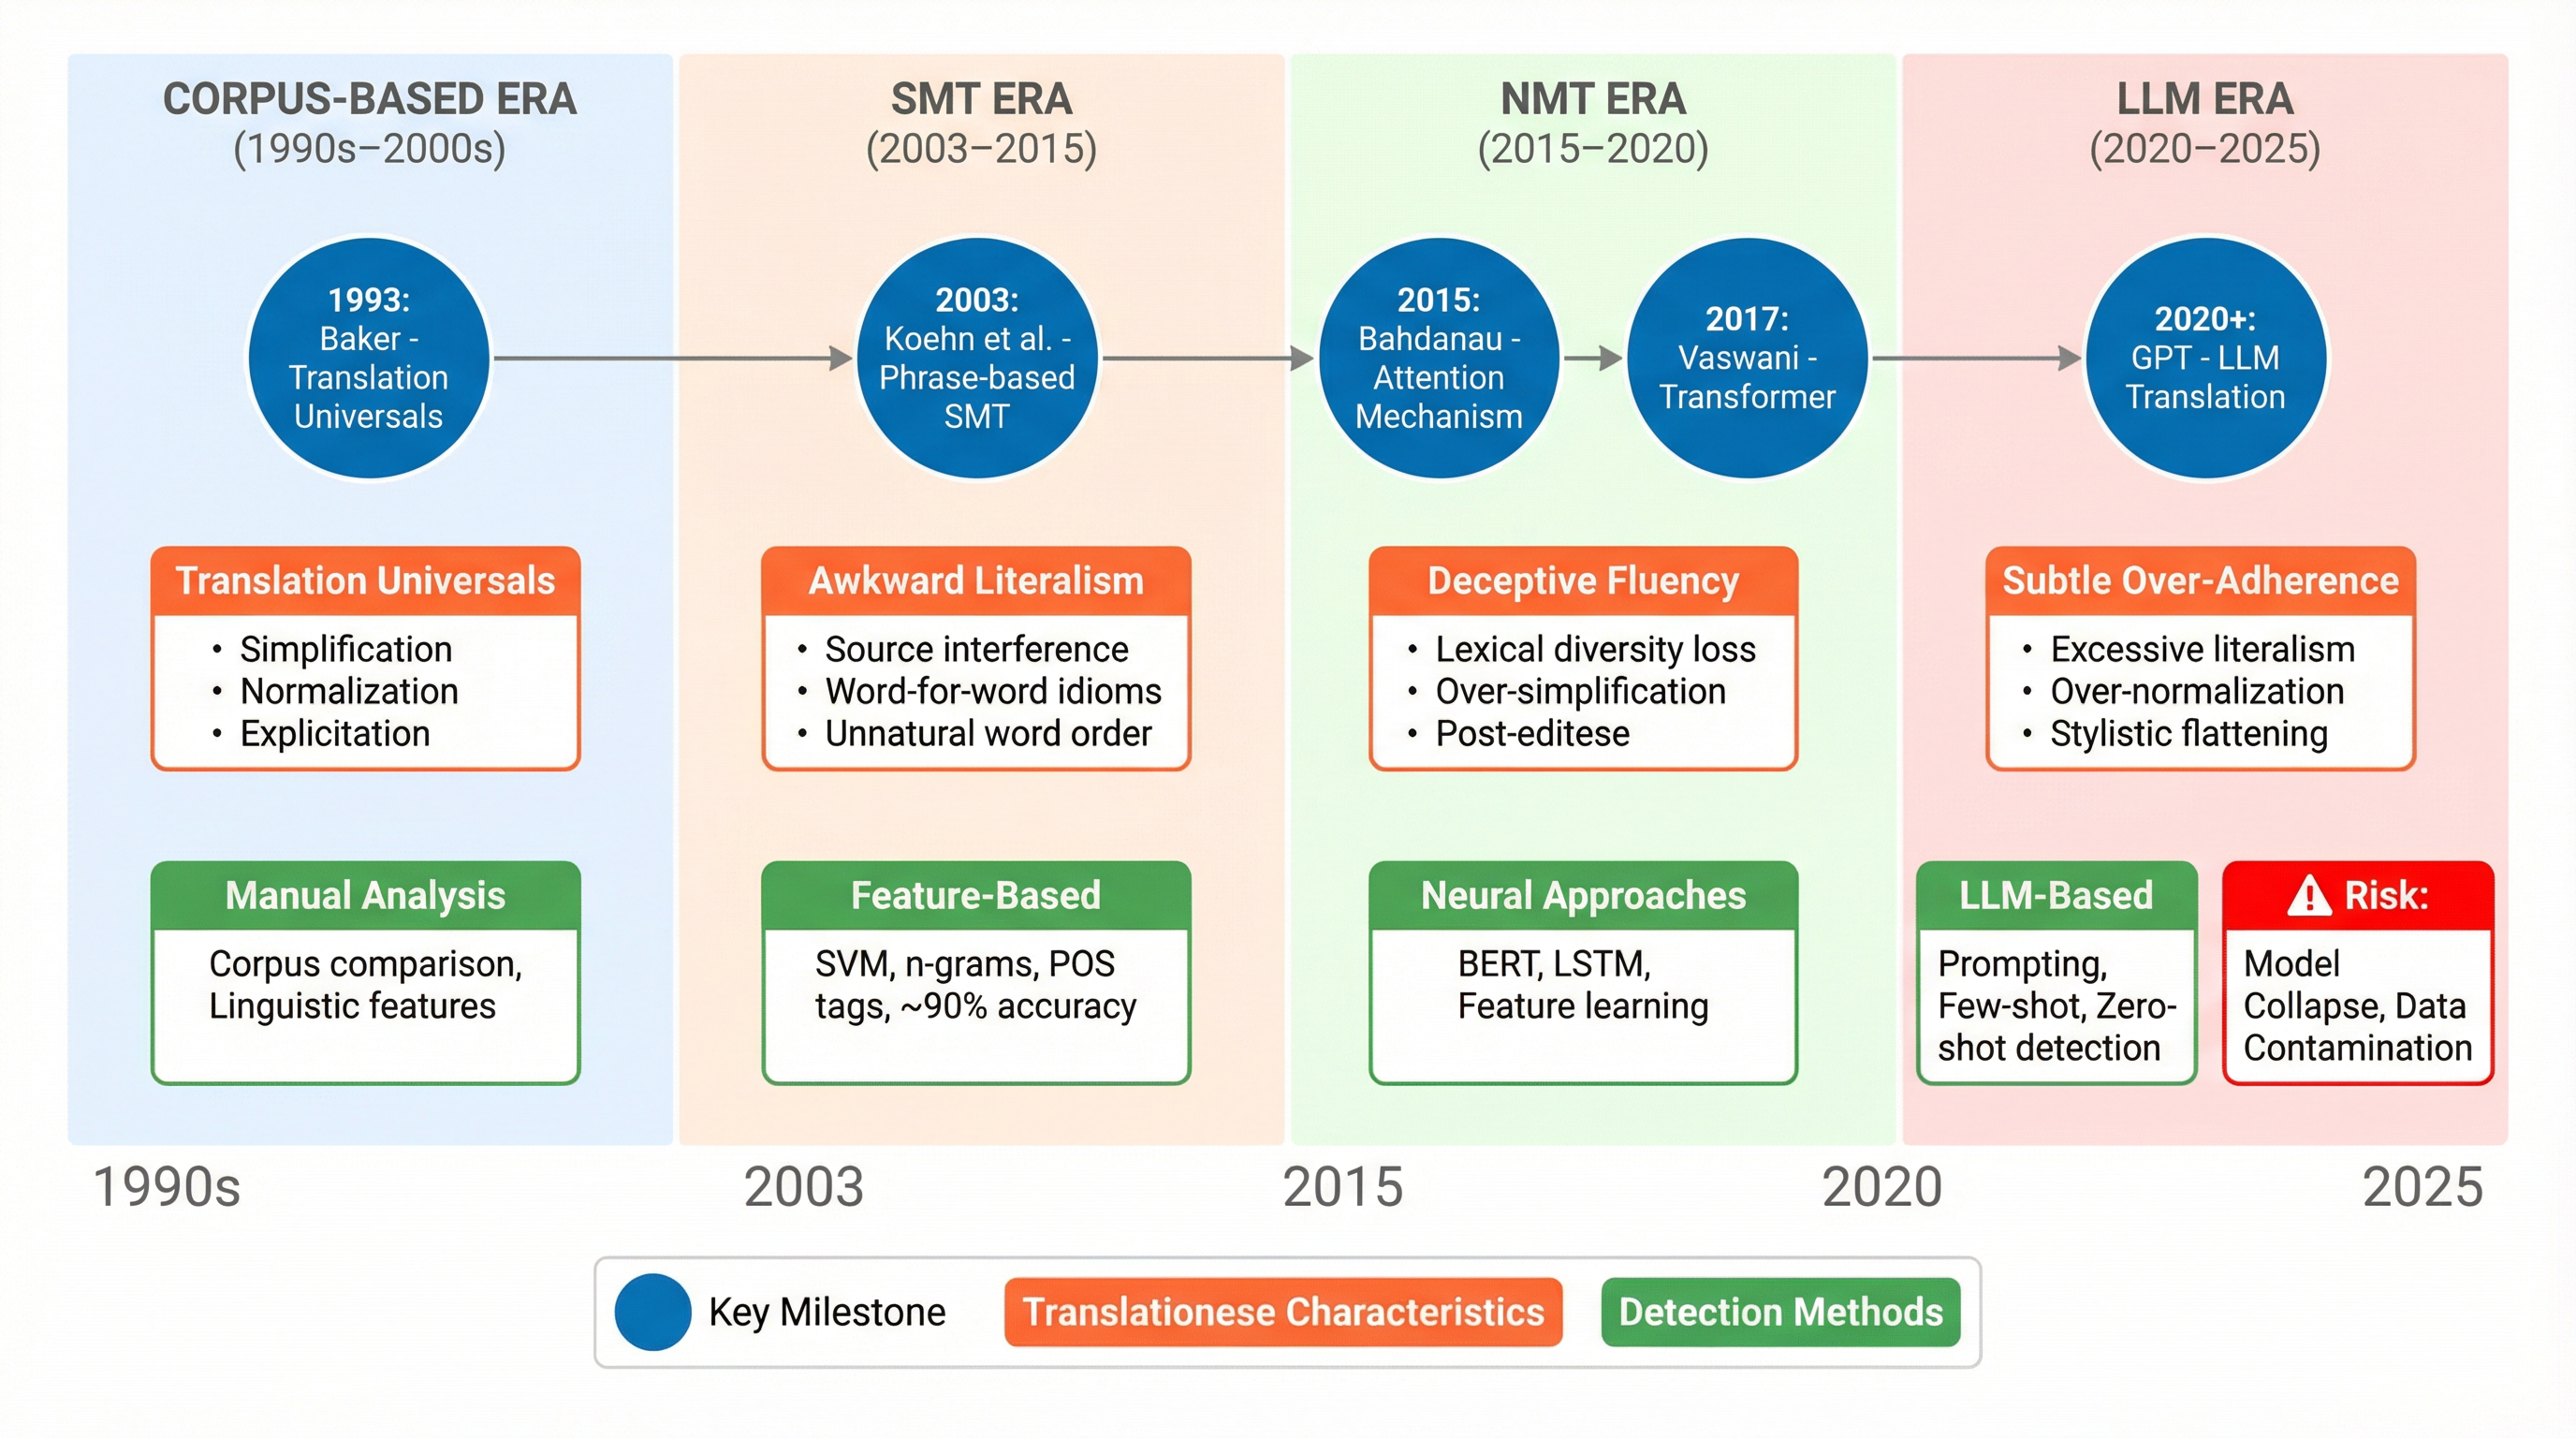
\includegraphics[width=\textwidth]{figure1_timeline_prototype.png}
\caption{Evolution of Machine Translation Paradigms and Translationese Characteristics (1990s--2025). This timeline illustrates the co-evolution of MT technologies and translationese over three decades. The top layer shows key technological milestones, the middle layer highlights dominant translationese features in each era, and the bottom layer traces detection methodology evolution. Note the progression from overt grammatical errors in SMT to subtle stylistic biases in LLMs, necessitating increasingly sophisticated detection approaches. The warning indicator highlights emerging risks of model collapse due to synthetic data contamination.}
\label{fig:mt-timeline}
\end{figure*}

\section{Background: The Evolving Nature of Machine Translationese}

Translationese refers to the distinctive linguistic characteristics that make translated text identifiably different from text originally written in the target language \cite{gellerstam1986translationese}. Initially studied in the context of human translation, these artifacts, or ``translation universals,'' include phenomena such as simplification (the tendency to use simpler language), normalization (the tendency to exaggerate features of the target language), and interference from the source language \cite{baker1993corpus}. As machine translation (MT) has evolved from rule-based systems to the sophisticated Large Language Models (LLMs) of today, the nature of machine translationese has co-evolved, shifting from overt grammatical errors to more subtle, systemic biases. To provide an initial insight into this evolution, we present classic examples of machine translationese from three distinct technological eras.

\subsection{The SMT Era: Awkward Literalism}

Statistical Machine Translation (SMT) systems, which dominated the field in the 2000s, operated by learning statistical alignments between phrases in a source and target language. While a significant leap forward, this phrase-based approach often resulted in outputs that were locally fluent but globally disfluent and awkward. The translationese of this era is characterized by literal, word-for-word translations of idioms and unnatural word order, making it easily noticeable.

\begin{quote}
\textbf{Source (Chinese):} \textit{他画蛇添足,结果把事情搞砸了。}

\textbf{Hypothetical SMT Output:} \textit{He drew a snake and added feet, and as a result messed up the matter.}

\textbf{Human Translation:} \textit{He ruined the matter by adding something superfluous.}
\end{quote}

In this example, the SMT system literally translates the idiom \textit{画蛇添足} (huà shé tiān zú), failing to capture its actual meaning of ruining something by doing more than is necessary. The output is a grammatically awkward and nonsensical sentence that clearly exposes the system's lack of deeper semantic understanding.

\subsection{The NMT Era: Deceptive Fluency}

Neural Machine Translation (NMT), particularly with the advent of the Transformer architecture, revolutionized the field by producing highly fluent and grammatically correct translations. However, this fluency can be deceptive. The translationese of the NMT era became more subtle, manifesting as a loss of lexical diversity, simplification of complex syntax, and a general tendency towards ``safe'' or generic language. As \citet{riley2020translationese} demonstrate, NMT models often produce outputs that achieve high automatic scores (like BLEU) but are disliked by human raters because they feel unnatural. The output is correct, but it often feels bland and lacks the richness of the source text.

\begin{quote}
\textbf{Source (German):} \textit{Die Gesetzgebung, ein labyrinthisches Geflecht von Klauseln und Unterklauseln, das über Monate kontroverser Debatten zusammengewoben wurde, wurde schließlich verabschiedet, wenn auch mit einem spürbaren Gefühl der müden Resignation aller beteiligten Parteien.}

\textbf{Hypothetical NMT Output:} \textit{The complex law was finally passed after a long debate, but all parties felt tired and resigned.}

\textbf{Human Translation:} \textit{The legislation, a labyrinthine tapestry of clauses and sub-clauses woven together over months of contentious debate, finally passed, albeit with a palpable sense of weary resignation from all parties involved.}
\end{quote}

Here, the NMT output is perfectly readable but has stripped the source text of its evocative vocabulary (``labyrinthisches Geflecht'' translated as ``complex law'' instead of ``labyrinthine tapestry'') and flattened its complex sentence structure. This simplification and normalization make the text less engaging and lose the stylistic nuance of the original author.

\subsection{The LLM Era: Subtle Over-Adherence}

Large Language Models (LLMs) represent the current state-of-the-art, capable of producing translations that are often indistinguishable from human-written text. The translationese of this era is even more insidious. It is characterized by excessive literalism, where the model adheres too closely to the source text's syntactic structure even when a more natural target-language construction exists, and over-normalization, where it smooths out unique stylistic choices in favor of highly probable, generic phrasing. \citet{li2025lost} systematically evaluate this phenomenon, showing that even powerful LLMs produce ``unexpected unnatural translations'' due to biases introduced during supervised fine-tuning.

\begin{quote}
\textbf{Source (Chinese):} \textit{少样本LLMs仍然落后于常规微调。}

\textbf{LLM Output (from \citet{li2025lost}):} \textit{Few-shot LLMs still lag behind vanilla fine-tuned models in the task.}

\textbf{Refined Human Translation:} \textit{Few-shot LLMs still lag behind vanilla fine-tuning.}
\end{quote}

In this example, cited directly from \citet{li2025lost}, the LLM output is overly literal. It translates ``常规微调'' (chángguī wēitiáo) as ``vanilla fine-tuned models in the task,'' which is a wordy and unnatural phrasing in English. The refined version, ``vanilla fine-tuning,'' is more concise and natural. This demonstrates the challenge of LLM-era translationese: it is not about what is wrong, but about what is lost in the subtle choices of phrasing and style.

These examples illustrate that as MT systems have become more powerful, machine translationese has not disappeared but has merely become more difficult to detect. Understanding this evolution is crucial for developing robust methods for identifying, evaluating, and managing its effects, a challenge that this survey aims to address.

\section{Identifying Translationese: Characterization and Detection}

This section surveys the evolution of methods for identifying machine translationese, tracing the progression from foundational corpus-based studies to modern neural approaches. We structure this review chronologically, highlighting how the understanding and detection of translationese have co-evolved with MT paradigms.

\subsection{Foundational Concepts from Corpus-Based Studies}

The systematic study of translationese originates from the field of Corpus-Based Translation Studies (CTS), which emerged in the 1990s. Before this, observations about the peculiar nature of translated text were largely anecdotal and confined to literary criticism. CTS provided a new paradigm, enabling researchers to analyze large electronic corpora of translated and non-translated texts to identify systematic, quantifiable differences \cite{laviosa1998corpus}. This empirical approach led to the formulation of several influential hypotheses about the nature of translation, often referred to as ``translation universals.''

One of the most prominent hypotheses is \textbf{simplification}, which posits that translated texts tend to be lexically and syntactically simpler than original texts. This can manifest in several ways, such as a lower type-token ratio (TTR), indicating less lexical diversity; shorter average sentence length; and a preference for more common words and grammatical structures \cite{baker1993corpus}. For example, a translator might subconsciously replace a rare, nuanced verb with a more generic one, or break up a long, complex sentence into several shorter ones to reduce cognitive load.

Another key hypothesis is \textbf{explicitation}, the tendency for translators to make implicit information in the source text more explicit in the target text. This can involve adding cohesive devices like conjunctions (e.g., ``however,'' ``therefore''), clarifying pronoun references, or spelling out cultural assumptions that would be obvious to a source-language reader but not to a target-language one. While explicitation can improve clarity, it can also lead to a more verbose and less natural-sounding text.

Finally, \textbf{normalization} (or conventionalization) suggests that translated texts tend to exaggerate the typical features of the target language, making them more ``normal'' than original texts. This can involve a preference for standard collocations, a tendency to avoid creative or unusual language, and a general regression to the mean of the target language's statistical properties. As \citet{gellerstam1986translationese} observed in his early work on Swedish novels translated from English, translated texts often feel ``flatter'' and less stylistically adventurous than their non-translated counterparts.

It is important to note that these hypotheses are not without their critics. Some scholars argue that they are not true ``universals'' but rather tendencies that are highly dependent on factors like the language pair, the direction of translation, and the translator's experience \cite{zanettin2013corpus}. A related concept, \textbf{interference} (or ``shining-through''), posits that many features of translationese are simply the result of the source language's structure being inappropriately carried over into the target language. Despite these debates, the concepts of simplification, explicitation, and normalization laid the crucial groundwork for all subsequent research into translationese, providing a conceptual vocabulary and a methodological toolkit that would later be adapted for the study of machine translation.

\subsection{Feature-Based Methods in the SMT Era}

The rise of Statistical Machine Translation (SMT) in the 2000s marked a pivotal moment for translationese research. For the first time, large quantities of machine-generated text were available for analysis, and the task of identifying translationese shifted from a descriptive, linguistic endeavor to a predictive, computational one. The central goal became to automatically distinguish between original text and translated text, a task that was formalized as a binary classification problem.

In this paradigm, a given text $x$ is classified as either belonging to the class $Y=1$ (translated) or $Y=0$ (original). The dominant approach was to use supervised machine learning models, particularly Support Vector Machines (SVMs), to learn a decision boundary between the two classes. An SVM learns a hyperplane defined by a weight vector $\mathbf{w}$ and a bias $b$ that best separates the data points. The classification of a new text $x$ is then given by:

$$ f(x) = \text{sign}(\mathbf{w}^T \phi(x) + b) $$

where $\phi(x) \in \mathbb{R}^d$ is a feature vector that represents the text $x$ in a $d$-dimensional space. The success of this approach hinged entirely on the quality of the hand-crafted features in $\phi(x)$.

Researchers developed a rich taxonomy of features designed to capture the subtle statistical artifacts of translationese. These can be broadly categorized as:

\begin{itemize}
    \item \textbf{Lexical Features:} These capture aspects of word usage. They include simple measures like n-gram frequencies (unigrams, bigrams, trigrams), which can reveal patterns of overuse or underuse of certain words and phrases. More sophisticated lexical features include TTR and its variants to measure lexical diversity, and the frequency of function words, which are often a strong indicator of translationese.
    \item \textbf{Syntactic Features:} These features are derived from the grammatical structure of the text. They often require parsing the text to obtain a syntax tree. Common syntactic features include the frequency of different part-of-speech (POS) tags and sequences, the depth of parse trees (as a measure of syntactic complexity), and the frequency of specific grammatical constructions (e.g., passive voice).
    \item \textbf{Information-Theoretic Features:} These features, such as perplexity and cross-entropy, measure how ``surprising'' a text is with respect to a language model trained on a large corpus of original text. The intuition is that translated text, due to its more conventional nature, will have a lower perplexity (i.e., be less surprising) than original text.
\end{itemize}

Using these features, researchers were able to build classifiers that could identify translationese with high accuracy, often exceeding 90\% \cite{baroni2006new, ilisei2010identifying}. This line of research also led to more nuanced insights. \citet{koppel2011translationese} introduced the concept of ``translationese dialects,'' showing that the features of translationese vary depending on the source language. Similarly, \citet{van2008source} demonstrated the existence of ``source language markers,'' specific features that betray the text's origin. This work was not purely academic; it had practical applications for improving SMT systems. For example, \citet{lembersky2013improving} showed that by adapting translation models to the specific characteristics of translationese, they could achieve significant improvements in translation quality.

\subsection{Neural Approaches in the NMT Era}

The transition from SMT to Neural Machine Translation (NMT) in the mid-2010s brought about another paradigm shift. NMT models, particularly those based on the Transformer architecture \cite{vaswani2017attention}, produced translations that were significantly more fluent and natural-sounding than their SMT predecessors. This had two major consequences for translationese research.

First, the nature of translationese itself became more subtle. The overt grammatical errors and awkward phrasing common in SMT outputs were largely eliminated. Instead, NMT translationese manifested as more nuanced biases, such as a loss of lexical diversity, a tendency towards more conservative language use, and a flattening of stylistic variation \cite{vanmassenhove2019getting}. This made detection more challenging, as the statistical signals were weaker.

Second, the research methodology shifted from \textbf{feature engineering} to \textbf{feature learning}. Instead of manually crafting features, researchers began to use deep neural networks, particularly pre-trained language models like BERT, to learn relevant features directly from the data. In this approach, the entire text is fed into the model, which then outputs a probability that the text is translated. \citet{pylypenko2021comparing} conducted a thorough comparison of feature-engineering and feature-learning approaches, finding that while neural models generally performed better, the combination of both often yielded the best results.

This shift also brought a new focus on \textbf{explainability}. Since neural models are often black boxes, researchers sought to understand \textit{what} features the models were learning to distinguish between original and translated text. Techniques like attention visualization and probing tasks were used to interpret the models' decisions. For example, \citet{amponsah2022explaining} used attention mechanisms to show that neural models were implicitly learning some of the same syntactic and lexical features that had been hand-crafted in the SMT era.

The NMT era also saw the emergence of new concepts. \citet{toral2019post} introduced the term ``post-editese'' to describe the language produced when humans post-edit machine translation output. He argued that post-editese is a distinct variety of language, different from both human translation and raw MT, and that it represents an ``exacerbated translationese.'' Furthermore, \citet{riley2020translationese} argued that in the context of large multilingual NMT models, translationese can be thought of as a distinct ``language'' in its own right, with its own grammar and vocabulary. This perspective has important implications for how we train and evaluate multilingual models.

\subsection{Emerging Patterns and Detection Challenges in the LLM Era}

The advent of Large Language Models (LLMs) has once again reshaped the landscape of translationese research. While the examples in Section~2 illustrate the \textit{characteristics} of LLM translationese (e.g., excessive literalism), this section focuses on the \textit{methodological challenges and opportunities} for its identification. The near-human fluency of LLM outputs renders traditional feature-based and even some neural classification methods less effective, necessitating a shift in research focus from binary classification to more nuanced, fine-grained stylistic analysis \cite{li2025how,wang2024benchmarking}.

One of the primary challenges is that LLM-generated translationese often lacks the overt statistical artifacts that characterized earlier MT paradigms. The powerful generative capabilities of models like GPT-4 can smooth over many of the lexical and syntactic irregularities that feature-based systems relied on. Consequently, the research community has begun to explore new avenues for detection.

A growing body of work has turned to \textbf{zero-shot and few-shot detection}, where LLMs themselves are leveraged as detectors. This approach moves away from training dedicated classifiers on large labeled datasets. Instead, it involves crafting sophisticated prompts that ask an LLM to evaluate a given text for signs of translationese, or to compare it against a reference text for stylistic divergence. For example, a prompt might ask the model to rate a sentence on a scale of 1 to 10 for ``naturalness'' or ``idiomaticity,'' providing a more continuous measure of quality than a simple binary label \cite{dabre2024pretraining}.

Parallel to this development, the focus is shifting from a binary ``translated vs. original'' task to a more fine-grained \textbf{stylistic analysis}. Researchers are developing metrics to quantify specific aspects of translationese, such as the degree of literalism or the loss of stylistic richness. \citet{li2025how} propose methods to measure ``literalism scores'' by analyzing semantic and syntactic parallelism between the source and target texts. This allows for a more detailed characterization of translationese, not just its presence or absence. This shift is critical, as the goal is often not just to detect translationese, but to understand its specific nature and its impact on the reader's experience.

Another emerging research direction examines \textbf{cross-model variations} in translationese. Different LLMs, and even different versions of the same model, exhibit distinct translationese patterns. These variations can be traced back to differences in training data (e.g., the proportion of human-written vs. machine-generated text), model architecture, and fine-tuning strategies (e.g., SFT vs. RLHF). \citet{wang2024benchmarking} provide a comprehensive comparison of translationese across various popular LLMs, revealing that no single model is universally superior in avoiding translationese. This line of research is crucial for developing model-specific detection and mitigation strategies.

The rise of LLMs has also highlighted the importance of considering the \textbf{multilingual context}. The translationese produced by LLMs can vary significantly depending on the language pair, with low-resource languages often exhibiting more pronounced artifacts. \citet{jourdan2025translationese} explore the fairness implications of this phenomenon, arguing that translationese can perpetuate and even amplify existing biases in training data. This underscores the need for detection methods that are not only accurate but also equitable across different languages and cultural contexts.

The LLM era has thus pushed the field of translationese identification beyond simple binary classification. The new frontier lies in developing nuanced, explainable, and equitable methods for stylistic analysis, often leveraging the very models that produce the translationese in the first place. Future work will likely focus on real-time detection systems, automated quality assessment, and the integration of translationese detection into the core of MT evaluation and development pipelines.

\section{Evaluating its Impact: Quality, Bias, and Fairness}

While the previous section focused on identifying translationese, this section explores its consequences. The presence of these linguistic artifacts is not merely a theoretical curiosity; it has profound and often detrimental effects on the entire machine translation ecosystem, from the evaluation of translation quality to the perpetuation of societal biases. We examine these impacts through three critical lenses: the distortion of quality metrics and the debate over human parity; the risk of algorithmic bias and homogenization; and the misrepresentation of gender and other demographic information.

\subsection{Effects on Translation Quality and Human Parity}

The relationship between translationese and perceived translation quality is complex and often paradoxical. Intuitively, one might assume that text laden with unnatural artifacts is inherently of lower quality. While this is often true from a human perspective, the metrics used to automatically evaluate machine translation systems can tell a different, more misleading story. This discrepancy has been a central challenge in MT evaluation and has fueled a contentious debate over the concept of ``human parity."

A key issue is that translationese can artificially inflate automatic evaluation scores like BLEU. \citet{riley2020translationese} demonstrated this phenomenon by explicitly biasing an NMT model to produce more translationese. Counterintuitively, this led to an increase in BLEU scores while human evaluators rated the same output as lower in both fluency and adequacy. This ``gaming" of the metric occurs because translationese often relies on simpler, more frequent, and more predictable lexical choices. Since reference translations used in evaluation are themselves a form of translated text and often exhibit similar properties, a system that produces translationese is, in a sense, better at matching the statistical profile of the reference, even if the output is less natural to a native speaker.

This problem is at the heart of the controversy surrounding claims of ``human parity" in machine translation. Several high-profile studies have claimed that their MT systems perform on par with professional human translators. However, subsequent research has called these claims into question by highlighting the confounding role of translationese in the evaluation data. \citet{toral2018reassessing} and \citet{freitag2019translationese} conducted detailed re-evaluations of these claims, arguing that the test sets used were often composed of translated texts (e.g., news articles translated from another language) rather than original, natively-written texts. When an MT system is evaluated on its ability to reproduce human-generated translationese, achieving ``parity" does not mean the system can produce text indistinguishable from that of a native human writer; it only means it is good at mimicking the specific artifacts of human translation. As \citet{freitag2019translationese} argue, this is not a true test of native-level quality, leading them to recommend that such reverse-created test data be omitted from future evaluations.

Furthermore, \citet{freitag2019translationese} raised a critical methodological point regarding the statistical power of the tests used in these human parity studies. They noted that the very goal of such evaluations is to find no significant difference between human and machine outputs. However, if the statistical test has low power, it may fail to detect a real difference that exists (a Type II error), leading to a premature and unsubstantiated claim of parity. This highlights the need for larger sample sizes and more rigorous statistical methods in human evaluation to ensure that claims of parity are robust and meaningful.

In essence, the pervasive nature of translationese in both training and evaluation data creates a distorted ecosystem. It undermines the reliability of automatic metrics, complicates the interpretation of human evaluations, and makes the pursuit of ``human parity" a moving and often ill-defined target. Achieving true human-level quality requires not just matching reference translations, but generating text that is free of the subtle artifacts that betray its machine origins.

\subsection{Algorithmic Bias and Homogenization}

Beyond the immediate challenges to evaluation, translationese introduces a more insidious long-term risk: the gradual erosion of linguistic diversity. This phenomenon, often termed \textbf{homogenization}, describes the tendency of machine translation systems to produce outputs that are less varied and more conventional than human-written text. The models learn the statistical regularities of their training data---much of which is itself translationese---and regress towards a linguistic mean, smoothing over the stylistic richness, idiomatic expressions, and creative nuances that characterize authentic communication. \citet{sizov2024analysing} provide a comparative analysis of translation artifacts, showing that even advanced LLMs tend to produce text that is stylistically less adventurous than human translations. This creates a feedback loop: as more machine-generated text populates the internet, future models trained on this data will be exposed to an increasingly homogenized and impoverished linguistic environment.

This feedback loop can culminate in a catastrophic failure mode known as \textbf{model collapse}. As described by \citet{shumailov2024ai}, when generative models are recursively trained on data produced by previous versions of themselves, they can enter a degenerative process that leads to irreversible defects. The model begins to overfit to its own predictions, amplifying the most common patterns while forgetting the less frequent but often crucial details that reside in the tails of the original data distribution. In the context of translation, this means that rare words, complex syntactic structures, and subtle cultural references that were already underrepresented in the training data may disappear entirely from the model's generative capabilities. The result is a model that produces increasingly generic and bland output, eventually losing its ability to generate high-quality, diverse text.

The risk of model collapse is no longer a theoretical concern. With the proliferation of LLM-generated content online, the data scraped for training the next generation of models is inevitably contaminated with synthetic text. This poses an existential threat to the continued improvement of machine translation and other generative AI technologies. The very process that has driven their success---scaling up training on vast quantities of web data---may become their undoing. This underscores the critical importance of identifying and filtering translationese, not just for evaluating individual translations, but for preserving the health and diversity of the digital linguistic ecosystem upon which future models will depend.

\subsection{Gender and Demographic Representation}

The homogenizing effect of translationese extends beyond stylistic variation to the very representation of people. Translation models, in their tendency to simplify and normalize, often erase social and demographic diversity, defaulting to the most statistically common or unmarked forms. This has the most pronounced and well-documented consequences in the domain of gender.

Gender bias in machine translation is a long-standing problem. In many languages, gender is a grammatical category, and translating from a language with less grammatical gender (like English) to one with more (like French or Spanish) requires the model to make a choice. When the source text is ambiguous (e.g., "a doctor"), models trained on biased data will often default to the stereotypical gender, typically masculine \cite{vanmassenhove2019getting}. Translationese exacerbates this issue; the drive towards normalization reinforces the statistical dominance of masculine forms in the training corpus, making it even less likely for the model to produce gender-inflected outputs that challenge societal stereotypes.

The challenge has become more acute with the growing recognition of non-binary gender identities and the push for more inclusive language. The artifacts of translationese---simplification and conservatism---are fundamentally at odds with the linguistic innovation required to represent these identities fairly. Recent work has shown that even state-of-the-art LLMs struggle with this task. \citet{jourdan2025fairtranslate} introduced FairTranslate, a dataset specifically designed to evaluate non-binary gender biases in English-to-French translation. Their evaluation of several leading LLMs revealed ``substantial biases in gender representation,'' highlighting that models often fail to correctly translate inclusive language like the singular `they' or neopronouns.

This failure is not merely a technical shortcoming; it is a direct consequence of the models optimizing for statistical likelihood over social fairness. The linguistic patterns associated with inclusive language are, by definition, less frequent in the vast corpora of historical text used for training. A model guided by the principles of translationese will naturally see these patterns as noisy, low-probability outliers and will attempt to ``correct" them by reverting to more common, binary gender forms. The impact of translationese, therefore, is not just a matter of stylistic fidelity but of social equity. It can render certain demographic groups invisible and perpetuate harmful stereotypes, amplifying existing societal biases rather than mitigating them.

While gender is the most studied axis, this problem extends to other demographic characteristics. The translation of culturally specific honorifics, dialects, and sociolects is similarly flattened by the homogenizing pressure of translationese. For low-resource languages and cultures, which are already underrepresented in training data, this effect is even more severe. The result is a digital linguistic landscape that is not only less diverse but also less equitable, reflecting a narrow, statistically dominant worldview at the expense of marginalized communities.

\section{Managing its Effects: Mitigation and Application}

As the understanding of translationese has matured, research has shifted from merely identifying its presence to actively managing its effects. This section surveys the strategies developed to mitigate the negative impacts of translationese—such as quality degradation and bias—as well as emerging methods that leverage the unique properties of translationese for positive applications.

\subsection{Data-Centric Strategies}

Data-centric approaches focus on the composition and curation of training corpora to control the influence of translationese artifacts. These methods are based on the insight that MT models are highly sensitive to the linguistic properties of their input data.

\textbf{Filtering and Weighting:} A primary strategy involves identifying and either removing or down-weighting translated text within training corpora. \citet{lembersky2013improving} pioneered this approach in the SMT era, demonstrating that translation models trained exclusively on original (non-translated) text consistently outperformed those trained on translationese, even when the latter were larger. They proposed adapting the translation model to the specific characteristics of the target domain's original text. In the NMT era, this has evolved into more sophisticated data selection techniques that use translationese classifiers to filter out low-quality synthetic data or to prioritize human-authored text \cite{pylypenko2021comparing}.

\textbf{Synthetic Data Management:} The widespread use of back-translation—generating synthetic parallel data by translating monolingual target-language text into the source language—has introduced a new layer of complexity. While back-translation significantly improves fluency, it also introduces systematic artifacts. \citet{riley2020translationese} addressed this by using tags to distinguish between authentic and synthetic data. This allows the model to learn the distinction and avoid propagating the artifacts of the synthetic source into the target output.

\textbf{Structural Restoration:} Some researchers have proposed frameworks to explicitly ``undo'' the simplification effects of translation. \citet{chen2012simplification} introduced a Simplification-Translation-Restoration framework for cross-domain SMT. This approach first simplifies the source text to make it easier to translate and then applies a restoration step to recover the complex stylistic and structural features of the original domain, effectively mitigating the flattening effect of the MT process.

\subsection{Model-Centric Strategies}

Model-centric strategies involve architectural or procedural changes to the MT systems themselves to reduce the generation of translationese.

\textbf{Fine-tuning and Supervised Training:} The way models are trained, particularly during the supervised fine-tuning (SFT) phase, has a significant impact on translationese. \citet{li2025lost} argue that the common practice of SFT on high-quality human translations can inadvertently encourage ``literalism'' in LLMs, as the models learn to over-rely on the source text's structure. They suggest that mitigation requires more diverse training objectives that reward stylistic naturalness over strict structural adherence. Similarly, \citet{jourdan2025translationese} explore fine-tuning strategies to reduce the bias and normalization effects that often lead to the erasure of inclusive language and non-binary gender representation.

\textbf{In-Context Learning and Prompting:} For LLMs, the flexibility of in-context learning (ICL) offers a powerful tool for mitigation. By providing the model with examples of both literal (translationese) and natural human translations, or by explicitly instructing the model to avoid specific artifacts like over-normalization, researchers have shown that the ``naturalness'' of the output can be significantly improved \cite{wang2024benchmarking}. This approach allows for real-time mitigation without the need for expensive re-training.

\textbf{Decoding and Inference-Time Constraints:} Adjustments to the decoding process can also help. Techniques like nucleus sampling or beam search with length penalties can be tuned to favor more diverse and less predictable lexical choices, counteracting the simplification and normalization tendencies of the model. Furthermore, incorporating translationese-aware quality metrics directly into the decoding loop can guide the model towards more human-like outputs.

\subsection{Leveraging Translationese: Positive Applications}

While often viewed as a negative byproduct, translationese possesses unique properties that can be leveraged for specific computational tasks.

\textbf{Low-Resource Translation:} In scenarios where authentic human-written parallel data is scarce, translationese—particularly in the form of synthetic data—can be a vital resource. \citet{dabre2024pretraining} demonstrate that pre-training on large amounts of machine-generated (and thus translationese-heavy) text can provide a crucial foundation for low-resource languages, which can then be refined with a small amount of high-quality human data. In this context, translationese acts as a ``stepping stone'' to improve basic translation capabilities.

\textbf{Translationese as a Stylistic Pivot:} \citet{riley2020translationese} propose a novel perspective: treating translationese as a distinct ``language'' or stylistic variety within a multilingual model. By using language tags to explicitly mark translationese, they show that a model can learn to translate \textit{into} or \textit{away from} the translationese style. This not only improves the model's understanding of different linguistic varieties but also allows users to select the desired level of naturalness at inference time.

\textbf{Quality Estimation and Evaluation:} The very artifacts that define translationese can serve as valuable signals for quality estimation (QE). If an MT output exhibits strong markers of translationese (e.g., excessive literalism or extreme simplification), it can be flagged as potentially low-quality or in need of human post-editing. This transforms the detection of translationese from a purely analytical task into a practical tool for monitoring and improving the output of production MT systems \cite{toral2018reassessing, sizov2024analysing}.

\section{Future Directions and Open Problems}

Despite decades of research, translationese remains a dynamic and evolving field. The shift towards large-scale generative models has introduced new complexities that require interdisciplinary solutions.

\subsection{Mitigating the Recursive Loop: Data Provenance and Watermarking}

As the proportion of machine-generated text on the internet grows, the risk of \textbf{model collapse} becomes an existential threat to future MT development \cite{shumailov2024ai}. A critical future direction is the development of robust \textbf{data provenance} techniques. Identifying translationese will no longer be just a stylistic exercise but a prerequisite for data curation. Future research must focus on:
\begin{itemize}
    \item \textbf{Digital Watermarking:} Embedding imperceptible signals in MT output to facilitate its identification in future crawls.
    \item \textbf{High-Precision Classifiers:} Developing detection systems that can distinguish between human-generated translationese and machine-generated artifacts with high reliability. This includes moving beyond simple lexical features towards information-theoretic measures, such as entropy analysis, to quantify the "predictability" and "richness" of translated text \cite{wang2025assessing}.
    \item \textbf{Authentic Data Recovery:} Exploring methods to "de-bias" or "un-flatten" synthetic text to recover the original linguistic richness of the source domain.
\end{itemize}

\subsection{Translationese in Cross-Lingual Transfer and Zero-Shot Learning}

The role of translationese in \textbf{zero-shot and low-resource settings} remains under-explored. While current work suggests that translationese can serve as a useful pivot \cite{dabre2024pretraining, riley2020translationese}, it also risks propagating systemic biases into languages where authentic parallel data is nearly non-existent. Future work should investigate whether translationese artifacts act as a "universal pivot language" that facilitates transfer, or if they create a "linguistic ceiling" that prevents models from ever reaching native-level proficiency in low-resource contexts. Understanding the trade-off between the \textit{utility} of synthetic data and the \textit{fidelity} of the resulting output is a major open problem.

\subsection{Human-in-the-Loop: Post-Editese and Interactive Mitigation}

The interaction between human translators and MT systems introduces a specific variety of translationese known as \textbf{post-editese} \cite{toral2019post}. As interactive MT and real-time suggestion systems become standard in the translation industry, the boundary between human and machine creativity is blurring. Open problems include:
\begin{itemize}
    \item \textbf{Cognitive Load and Priming:} How does exposure to MT-generated translationese prime human translators to produce more literal or simplified output?
    \item \textbf{Interactive Correction:} Developing systems that can detect translationese in real-time and suggest more "natural" or "idiomatic" alternatives to the user, effectively acting as a stylistic assistant rather than just a translation engine.
    \item \textbf{Long-Form Consistency:} Moving beyond sentence-level artifacts to address translationese in discourse structure, document-level coherence, and multimodal contexts (e.g., video subtitling).
\end{itemize}

\section{Conclusion}

This survey has traced the evolution of translationese research from its roots in descriptive translation studies to its current status as a central challenge in the era of Large Language Models. What was once viewed primarily as a set of interesting linguistic universals—simplification, normalization, and interference—has become a critical factor in the quality, fairness, and long-term sustainability of machine translation systems.

We have seen that while neural architectures have achieved unprecedented levels of fluency, they have not eliminated translationese; rather, they have transformed it into a more subtle and insidious phenomenon. The artifacts produced by modern models, while less overt than the "broken" output of the past, continue to distort evaluation metrics, perpetuate demographic biases, and threaten the diversity of our digital linguistic ecosystem.

However, translationese is not merely a problem to be solved; it is also a powerful lens through which we can understand the inner workings of our models and the nature of human translation itself. By treating translationese as a distinct stylistic variety, we can develop more flexible MT systems, improve low-resource translation, and create more effective tools for quality estimation.

As we move forward, the goal of machine translation must shift from achieving statistical "parity" with human-generated translationese to pursuing \textbf{linguistic authenticity}. This requires a move away from data-hungry, likelihood-based optimization towards models that are stylistically aware, culturally sensitive, and capable of preserving the rich diversity of human expression. The study of translationese will remain at the heart of this endeavor, providing both the diagnostic tools and the conceptual framework for building the next generation of truly natural translation systems.

\bibliography{translationese}
\bibliographystyle{acl_natbib}

\end{document}


